% !TEX root = ../practicas_geogebra.tex
% Author: Alfredo Sánchez Alberca (asalber@ceu.es)
\chapter{Introducción a Geogebra}

\section{Introducción}
La gran potencia de cálculo alcanzada por los ordenadores en las últimas décadas ha convertido a los mismos en poderosas herramientas al servicio de todas aquellas disciplinas que, como las matemáticas, requieren cálculos largos y complejos.

Geogebra\footnote{Esta practica está basada en la versión 6.1 de Geogebra Clásico} es uno de los programas de cálculo numérico y simbólico más utilizados.
Aparte de sus capacidades el cálculo numérico, vectorial y matricial, también puede realizar representaciones gráficas, lo cual permite resolver multitud de problemas de Álgebra, Análisis, Cálculo, Geometría e incluso Estadística, de manera interactiva.
La ventaja de Geogebra frente a otros programas habituales de cálculo como Mathematica, Mapple o MATLAB, radica en su sencillez y simplicidad de uso, y en que es software libre, por lo que puede instalarse sin coste alguno e incluso modificarse.

\begin{center}

\includegraphics[scale=0.8]{img/introduccion/geogebra-logo}
\end{center}

El programa puede descargarse de las página web \url{https://www.geogebra.org}.
En esta web existe también una versión en linea del programa que permite usarlo como una aplicación web sin necesidad de instalarlo en el ordenador.
Esta web dispone también de multitud de tutoriales y recursos educativos a disposición de los usuarios.
De hecho, cualquier usuario puede registrarse y subir a esta web actividades desarrolladas con Geogebra.

El objetivo de esta práctica es introducir al alumno en la utilización de este programa, enseñándole a realizar las operaciones básicas más habituales en Cálculo.

\section{Arranque}
Como cualquier otra aplicación de Windows, para arrancar el programa hay que pulsar sobre la opción correspondiente del menú \menu{Inicio>Programas}, o bien sobre el icono de escritorio 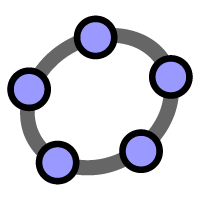
\includegraphics[scale=0.04]{img/introduccion/geogebra-icon}.

Cuando el programa arranca, en la pantalla aparece la ventana de inicio del programa (figura \ref{g:ventana-inicio}), que nos permite seleccionar distintos entornos de trabajo o \emph{Apariencias}.

\begin{figure}[h!]
\begin{center}
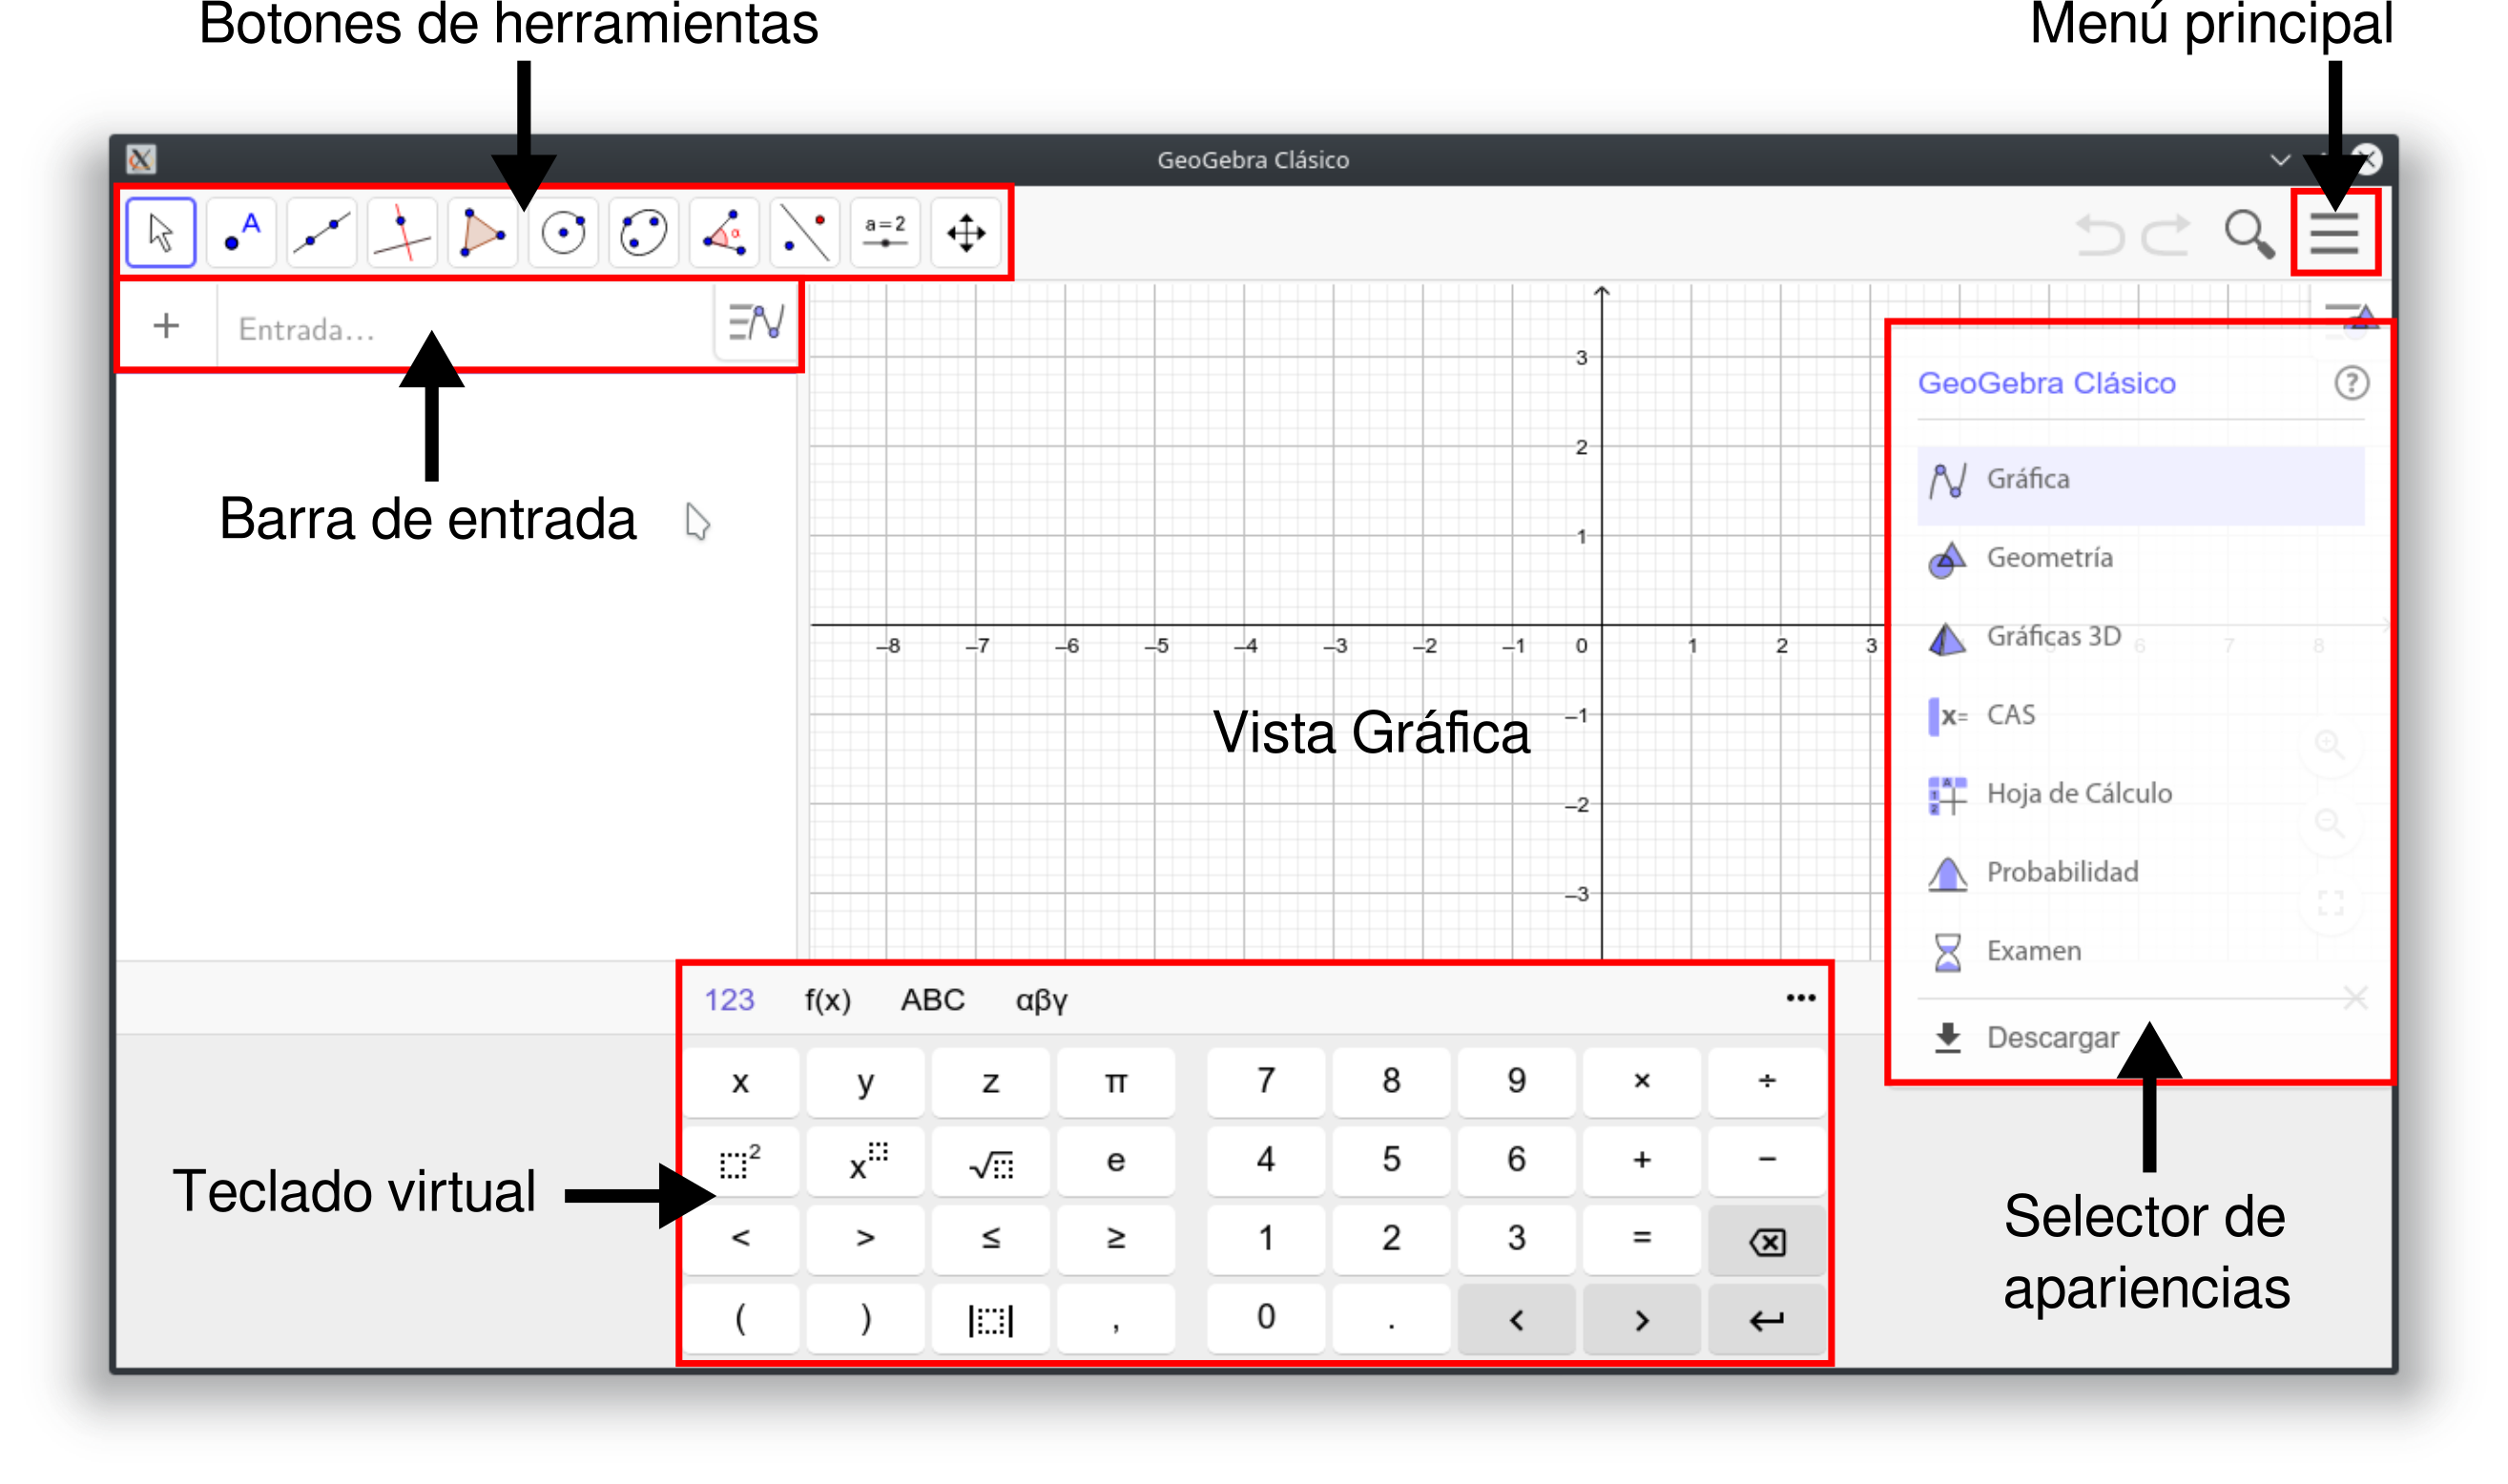
\includegraphics[width=\textwidth]{img/introduccion/start-window}
\caption{Ventana principal de Geogebra.} \label{g:ventana-inicio}
\end{center}
\end{figure}

\section{Vistas}
Geogebra dispone de varias ventanas de trabajo que se denominan \emph{Vistas} y de distintos entornos de trabajo llamados \emph{Apariencias} que combinan distintas vistas.
Tanto las vistas como las apariencias se pueden activar en el menú principal de Geogebra que aparece en la esquina superior derecha.
Las vistas más importantes que utilizaremos a lo largo de estas prácticas son:
\begin{description}
\item[Vista Algebraica] 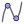
\includegraphics[scale=0.03]{img/introduccion/algebraic-view-icon} Esta permite realizar construcciones algebraicas y geométricas.
      Dispone una \field{Barra de Entrada} donde se pueden introducir comandos y expresiones algebraicas.
      Esta vista aparece activa por defecto cuando arranca el programa.
\item[Vista Gráfica] 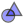
\includegraphics[scale=0.03]{img/introduccion/graphics-view-icon} Esta vista permite representar objetos geométricos en el plano real.
      Junto a la vista algebraica, esta vista también aparece activa por defecto cuando arranca el programa.
\item[Vista Gráfica 3D] 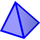
\includegraphics[scale=0.3]{img/introduccion/3d-graphics-view-icon} Esta vista permite representar objetos geométricos en el espacio real.
      Esta vista no aparece por defecto cuando arranca el programa, así que hay que activarla cuando se necesite.
\item[Vista CAS] 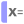
\includegraphics[scale=0.03]{img/introduccion/cas-view-icon} (Computer Algebra System) Esta vista permite realizar cálculos simbólicos. Dispone de una \field{Barra de Entrada} similar a la vista Algebraica donde se pueden introducir comandos y expresiones matemáticas y evaluarlas.
      Esta vista no aparece por defecto cuando arranca el programa, pero \emph{será la que más utilizaremos durante las prácticas.}
\end{description}


\section{Edición de expresiones en la \field{Vista CAS}}
Antes de realizar cualquier cálculo sobre una expresión matemática, lo primero es escribir dicha expresión y aprender a manipularla.


\subsection*{Introducción de expresiones}
Para introducir una expresión se utiliza \field{Barra de Entrada} de la \field{Vista CAS} (figura~\ref{g:barra-entrada}).

\begin{figure}[h!]
\begin{center}
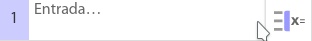
\includegraphics[scale=0.6]{img/introduccion/input-bar}
\caption{Barra de entrada de expresiones.} \label{g:barra-entrada}
\end{center}
\end{figure}

La \field{Barra de Entrada} permite introducir expresiones matemáticas, comandos y también anotaciones de texto.
En estas expresiones podemos introducir números, letras romanas, letras griegas, operadores matemáticos y cualquier símbolo matemático que aparece en el teclado virtual.
También permite la entrada de código \LaTeX\footnote{\url{https://www.latex-project.org/}} para formatear la expresiones.
Por ejemplo es posible escribir superíndices con el comando \command{\^{}} y subíndices con el comando \command{\_}.

Cuando se presiona la tecla \command{Enter} después de introducir una expresión matemática, Geogebra trata de evaluarla y muestra el resultado de la evaluación justo debajo de la expresión, o bien un aviso de error cuando hay algo mal escrito en la expresión.

Los operadores más habituales en la construcción de expresiones son los que aparecen en la siguiente tabla:

\begin{center}
\begin{tabular}{cc}
\tcrule
\textbf{Símbolo} & \textbf{Operador} \\
\command{+}      & suma              \\
\command{-}      & resta             \\
\command{*}      & producto          \\
\command{/}      & división          \\
\command{\^{}}   & potencia          \\
\bcrule
\end{tabular}
\end{center}

A la hora de escribir una expresión hay que tener en cuenta que Geogebra tiene establecido un orden de prioridad en la evaluación de los operadores.
En primer lugar evalúa las funciones y constantes predefinidas, después evalúa las potencias, después productos y cocientes (ambos con igual prioridad y de izquierda a derecha), y por último sumas y restas (ambas con igual prioridad y de izquierda a derecha).
Para forzar la evaluación de una subexpresión, saltándose el orden de prioridad, se utilizan paréntesis.
Así, como se ve en el siguiente ejemplo, dependiendo de cómo se introduzca una expresión pueden obtenerse resultados diferentes.


\begin{center}\renewcommand{\arraystretch}{2}
\begin{tabular}{cc}
\tcrule
\textbf{Expresión introducida} & \textbf{Expresión evaluada} \\
\texttt{4x-1/x-5}              & $4x-\dfrac{1}{x}-5$         \\
\texttt{(4x-1)/x-5}            & $\dfrac{4x-1}{x}-5$         \\
\texttt{4x-1/(x-5)}            & $4x-\dfrac{1}{x-5}$         \\
\texttt{(4x-1)/(x-5)}          & $\dfrac{4x-1}{x-5}$         \\
\bcrule
\end{tabular}
\end{center}

Cada vez que introducimos una expresión, esta aparece en la \field{Vista CAS} etiquetada con un número que permite identificarla.
Posteriormente, cada vez que queramos hacer referencia a dicha expresión podremos utilizar su identificador en lugar de volver a escribir la expresión.

Existen dos formas de referirse a una expresión anterior, que son la referencia estática y la referencia dinámica.
Para hacer una referencia estática debemos escribir el símbolo \# seguido el número que identifica la expresión, mientas que para hacer una referencia dinámica debemos escribir el símbolo \$ seguido del número que identifica la expresión.
Una referencia estática no cambiará la expresión donde se hace la referencia aún cuando la expresión original cambie, mientras que en una referencia dinámica, cuando cambie la expresión original, la expresión donde se hace la referencia reflejará ese cambio.

Es posible seleccionar cualquier expresión o subexpresión de la \field{Vista CAS} y copiarla y pegarla en la \field{Barra de Entrada}.


\subsection*{Introducción de anotaciones de texto}
Geogebra permite también la introducción de anotaciones o comentarios de texto en la \field{Barra de Entrada}.
Para ello hay que hacer clic con el botón derecho del ratón en la \field{Barra de Entrada} y seleccionar el menú \menu{Texto} del menú contextual que aparece.
Las anotaciones de texto son muy útiles para explicar los pasos que se dan en una construcción matemática o para interpretar los resultados.


\subsection*{Eliminación de expresiones}
Por supuesto, es posible eliminar una expresión de la \field{Vista CAS}.
Para ello solo hay que ir a la línea que contiene la expresión que se quiere eliminar y hacer clic en el botón 
\includegraphics[scale=0.035]{img/introduccion/bin-button.png} o hacer clic con el botón derecho del ratón y seleccionar el menú \menu{Eliminar fila} del menú contextual que aparece.

Si cometemos un error introduciendo una expresión o eliminándola, es posible deshacer las últimas operaciones o rehacerlas haciendo clic sobre los botones 
\includegraphics[scale=0.03]{img/introduccion/undo-button.png} o 
\includegraphics[scale=0.03]{img/introduccion/redo-button.png} respectivamente.


\subsection*{Definición de variables}
Para definir variables se pueden utilizar letras romanas o griegas.
Geogebra permite definir variables de más de una letra, de manera que la expresión \texttt{xy}, no se interpreta como el producto de la variable $x$ por la variable $y$, sino como la variable $xy$.
Además, distingue entre mayúsculas y minúsculas, así que no es lo mismo $xy$ que $xY$.


\subsection*{Definición de constantes y funciones}
Es posible definir constantes y funciones mediante el operador de definición \command{:=}.
Para definir una constante basta con escribir el nombre de la constante seguido de \command{:=} y el valor de dicha constante.
Por ejemplo para definir la constante de la aceleración de la gravedad, escribiríamos \command{g:=9.81}.

Por otro lado, para definir una función se escribe el nombre de la función seguido de la lista de variables de la misma separadas por comas y entre paréntesis; después se escribe \command{:=} y por último la expresión que define la función.
Así, por ejemplo, para definir la función que calcula el área de un triángulo de base $b$ y altura $h$, escribiríamos \command{a(b,h):=(b*h)/2} (ver figura~\ref{g:expresiones}).

Si hemos definido una función o una constante, y posteriormente cambiamos la definición, los cambios se verán reflejados en cualquier expresión donde aparezca la constante o la función, a no ser que hayamos hecho una referencia estática a ella.

Para eliminar la definición y dejar libre el nombre de la constante o función, por ejemplo \command{c}, se puede utilizar el comando \command{Eliminar(c)} o bien el comando \command{c:=}.

\subsection*{Funciones y constantes predefinidas}
Geogebra tiene ya predefinidas la mayoría de la funciones elementales y constantes que suelen utilizarse en los cálculos matemáticos.
La sintaxis de algunas de estas funciones y constantes se muestra en la tabla~\ref{t:funciones-predefinidas}, aunque, muy a menudo, en lugar de utilizar dicha sintaxis se utilizan los operadores y constantes que aparecen en el teclado virtual.

\begin{table}[h!]
\centering
\begin{tabular}{cl}
\tcrule
\textbf{Sintaxis}   & \textbf{Constante o función}                 \\
\command{pi}        & El número $\pi=3.14159\ldots$                \\
\command{Alt+e}     & Constante de Euler $e=2.71828\ldots$         \\
\command{Alt+i}     & El número imaginario $i=\sqrt{-1}$           \\
\command{inf}       & Infinito $\infty$                            \\
\command{exp(x)}    & Función exponencial $e^x$                    \\
\command{log(a,x)}  & Función logarítmica con base $a$, $\log_a x$ \\
\command{ln(x)}     & Función logaritmo neperiano $\ln x$          \\
\command{sqrt(x)}   & Función raíz cuadrada $\sqrt{x}$             \\
\command{sen(x)}    & Función seno $\sin x$                        \\
\command{cos(x)}    & Función coseno $\cos x$                      \\
\command{tan(x)}    & Función tangente $\tan x$                    \\
\command{arcsin(x)} & Función arcoseno $\arcsin x$                 \\
\command{arccos(x)} & Función arcocoseno $\arccos x$               \\
\command{arctan(x)} & Función arcotangente $\arctan x$             \\
\bcrule
\end{tabular}
\caption{Sintaxis de algunas funciones elementales y constantes predefinidas en Geogebra.} \label{t:funciones-predefinidas}
\end{table}

\subsection*{Vectores y matrices}
Geogebra también permite la manipulación de vectores y matrices.
Para definir un vector se escriben sus coordenadas separadas por comas entre paréntesis.
Por ejemplo, para introducir el vector $(x,y,z)$ escribiríamos \command{(x,y,z)} (ver figura~\ref{g:expresiones}).
Si se quiere un vector columna se puede usar el comando \command{Vector((x,y,z))}.

Para definir una matriz se escriben sus elementos por filas, separados por comas y entre llaves.
Así, para introducir por ejemplo la matriz
\[
\left(
\begin{array}{ccc}
1 & 2 & 3 \\
a & b & c \\
\end{array}
\right)
\]
escribiríamos \command{\{\{1,2,3\},\{a,b,c\}\}} (ver figura~\ref{g:expresiones}).


\subsection*{Simplificación de expresiones}
Geogebra trata de simplificar las expresiones cuando las evalúa.
Por ejemplo, si se introduce $x+x$ el resultado será $2x$.
Si no se desea evaluar una expresión se puede cambiar al modo de conservar las entradas haciendo clic en el botón 
\includegraphics[scale=0.03]{img/introduccion/keep-input-button}.

Sin embargo al evaluar una expresión Geogebra no realiza simplificaciones más complejas como por ejemplo simplificar la expresión $\sen(x)^2+\cos(x)^2=1$.
Para ello dispone de tres comandos:
\begin{description}
\item[Simplifica] Es el comando más sencillo y trata de simplificar al máximo una función.
      Por ejemplo, el comando \command{Simplifica(sen(x)\^{}2+cos(x)\^{}2)} devolverá \result{1}.
\item[Desarrolla] Este comando permite desarrollar una expresión realizando los potencias, productos, cocientes, sumas y restas que se puedan.
      Por ejemplo, el comando \command{Desarrolla((x+1)\^{}2)} devolverá el resultado \result{x\^{}2+2x+1}.
\item[Factoriza] Este comando permite factorizar una expresión.
      Por ejemplo, el comando \command{Factoriza(x\^{}2+2x+1)} devolverá el resultado \result{(x+1)\^{}2}.
\end{description}

En cualquiera de estas simplificaciones, Geogebra trabaja por defecto en modo exacto y por eso devuelve expresiones fraccionarias.
Para obtener el valor de una expresión en modo aproximado, con decimales, hay que cambiar al modo de cálculo aproximado haciendo clic sobre el botón 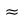
\includegraphics[scale=0.03]{img/introduccion/approximate-button}.
El número de cifras decimales se puede establecer en la configuración de Geogebra.

Por último, es posible sustituir cualquier variable de una expresión por un valor u otra expresión mediante el comando \command{Sustituye(<expresion>, <Lista de reemplazos>)}.
Por ejemplo, el comando \command{Sustituye(2x+y, x=2, y=1)} devolverá el resultado \result{5}.

\subsection*{Ecuaciones e inecuaciones}
Para definir ecuaciones en Geogebra hay que utilizar el símbolo de igualdad \command{=}.
Por ejemplo, el comando \command{2x-y=1} define la ecuación de una recta.

Y para definir inecuaciones en Geogebra hay que utilizar los símbolos de menor \command{<}, mayor \command{>}, menor o igual \command{<=} o mayor o igual \command{>=}.
Por ejemplo, el comando \command{x\^{}2+y\^{}2<=1} define el círculo de radio 1 centrado en el origen.

Para resolver ecuaciones e inecuaciones se utiliza el comando \command{Resuelve(<ecuaciones>)}.
Por ejemplo, el comando \command{Resuelve(x\^{}2-5x+4=0)} devolverá el resultado \result{\{x=1, x=4\}}.
Se pueden indicar además restricciones para las variables.
Por ejemplo, el comando \command{Resuelve(x\^{}2-5x+4=0, x>3)} devolverá únicamente la solución \result{\{x=4\}}.

Para resolver sistemas de ecuaciones hay que poner la lista de ecuaciones entre llaves.
Por ejemplo, el comando \command{Resuelve({2x+3=7, x-y=-1})} devolverá el resultado \result{\{x=3, y=2\}}.

Este comando también permite resolver inecuaciones.
Por ejemplo, el comando \command{Resuelve(3x-2<1)} devolverá el resultado \result{\{x<1\}}.


\section{Representaciones gráficas}
Uno de los puntos fuertes de Geogebra es su capacidad gráfica ya que permite representar multitud de objetos geométricos tanto en el plano como en el espacio real.

\subsection*{Representaciones gráficas en el plano real}
Para representar objetos geométricos en el plano real $\mathbb{R}^2$, Geogebra dispone de la \field{Vista Gráfica}.
Por defecto cualquier función que definamos en la \field{Vista CAS} aparecerá representada en esta vista.
Para representar otros objetos como constantes, ecuaciones o inecuaciones es necesario hacer clic sobre el círculo que aparece a la izquierda de la expresión (ver figura~\ref{g:vista-grafica}).
Para ocultar de nuevo el objeto en la \field{Vista Gráfica} basta con volver a hacer clic sobre ese círculo.

\begin{figure}[h!]
\begin{center}
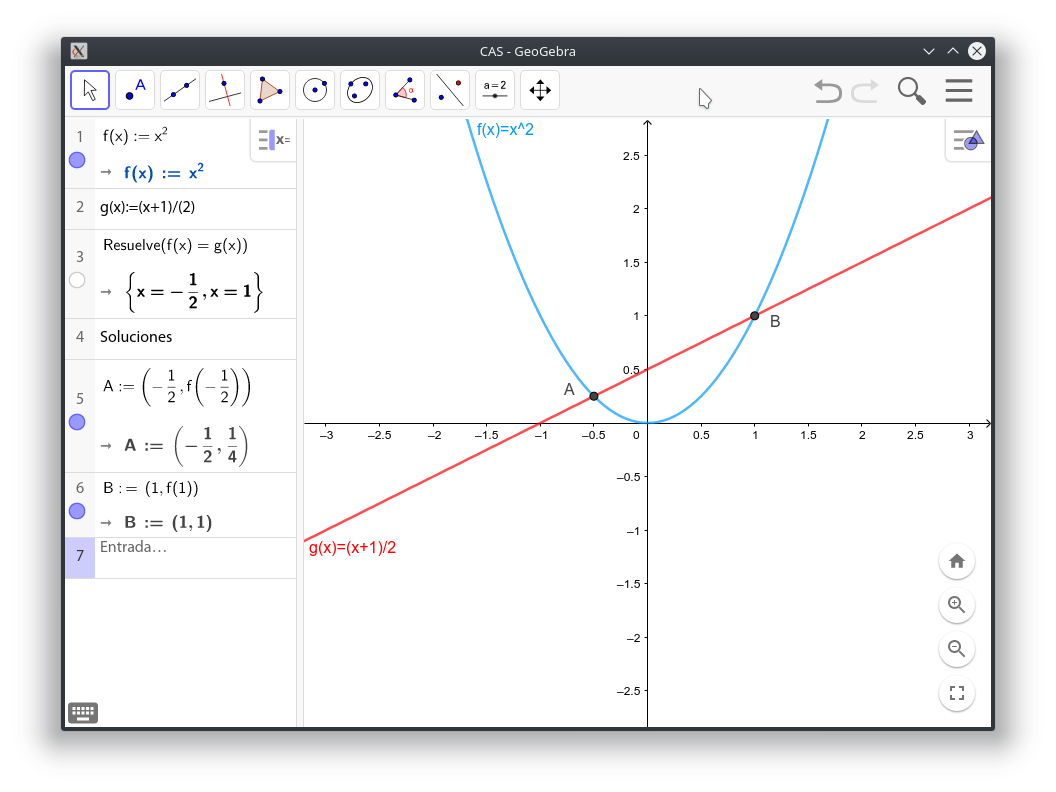
\includegraphics[width=\textwidth]{img/introduccion/graphic-view}
\caption{Representaciones gráficas en la \field{Vista Gráfica}.} \label{g:vista-grafica}
\end{center}
\end{figure}

Geogebra permite también la representación de funciones paramétricas definiendo el vector de las funciones coordenadas en función de un parámetro.
Por ejemplo, el comando \command{g(t):=(cos(t), 2sen(t)cos(t))} dibuja la curva que se muestra en la figura~\ref{g:curva-parametrica}.

\begin{figure}[h!]
\begin{center}
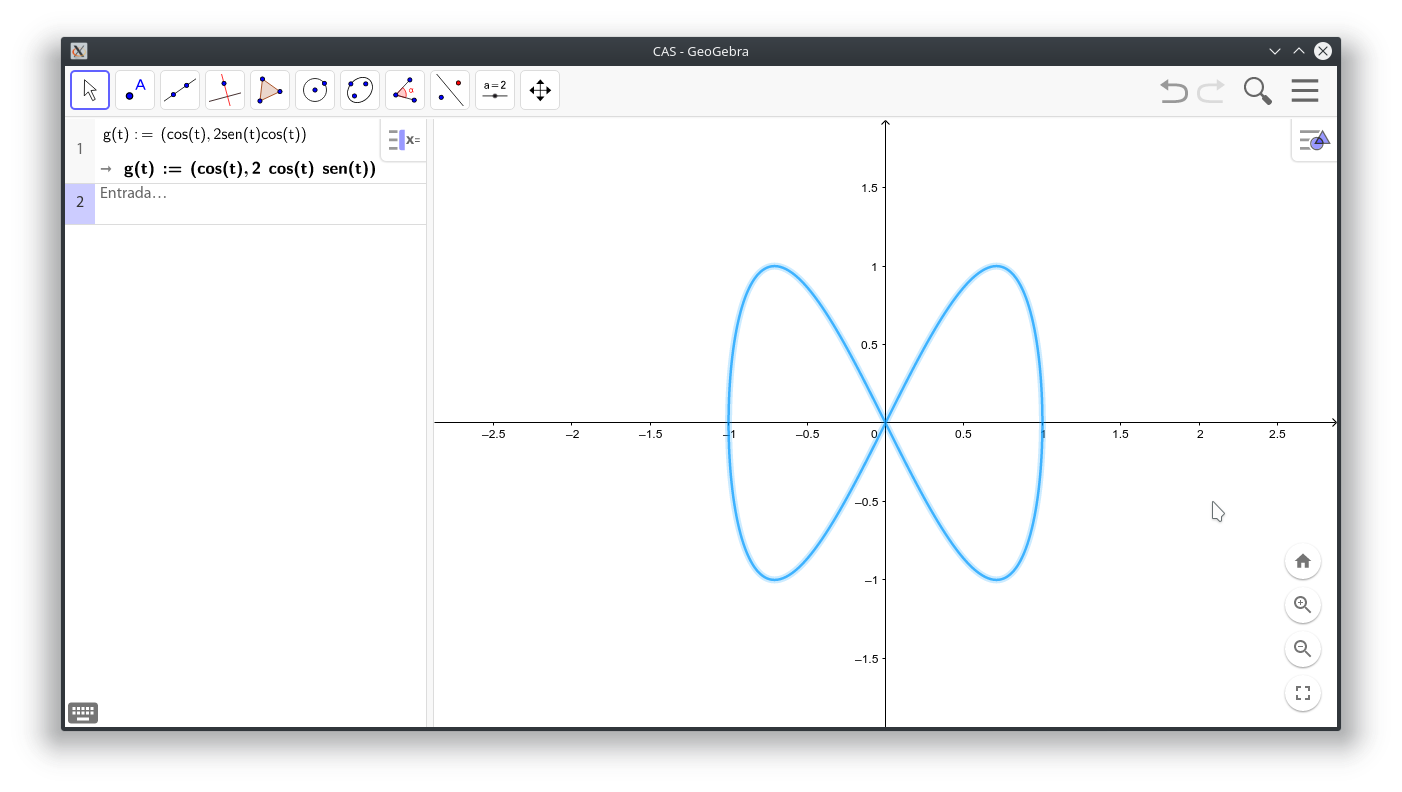
\includegraphics[width=\textwidth]{img/introduccion/parametric-curve}
\caption{Representación de una curva paramétrica en el plano.} \label{g:curva-parametrica}
\end{center}
\end{figure}

Es posible cambiar el aspecto de cualquier objeto geométrico haciendo clic con el botón derecho del ratón sobre él y seleccionando el menú \menu{Configuración} del menú contextual que aparece.
Esto abre un panel que permite cambiar el nombre del objeto, el color, el grosor o la transparencia del trazo, e incluso ponerle un rótulo que aparezca en la \field{Vista Gráfica} junto al objeto.

La \field{Vista Gráfica} aparece centrada en el origen de coordenadas por defecto, pero se puede hacer un zoom para acercar o alejar la vista haciendo clic en los botones 
\includegraphics[scale=0.03]{img/introduccion/zoom-in-button} y 
\includegraphics[scale=0.03]{img/introduccion/zoom-out-button} respectivamente.
También es posible desplazar la vista haciendo clic en cualquier posición y, sin soltar, desplazando el ratón.
Para volver a la vista original centrada en el origen de coordenadas, basta con hacer clic en el botón 
\includegraphics[scale=0.03]{img/introduccion/home-button}.


\subsection*{Representaciones gráficas en el espacio real}
Para representar objetos geométricos en el espacio real $\mathbb{R}^3$, Geogebra dispone de la \field{Vista Gráficas 3D}.

Por defecto cualquier función de dos variables que definamos en la \field{Vista CAS} aparecerá representada en esta vista.
Para representar otros objetos como ecuaciones es necesario hacer clic sobre el círculo que aparece a la izquierda de la expresión (ver figura~\ref{g:vista-grafica-3D}).
Para ocultar de nuevo el objeto en la \field{Vista Gráfica} basta con volver a hacer clic sobre ese círculo.

\begin{figure}[h!]
\begin{center}
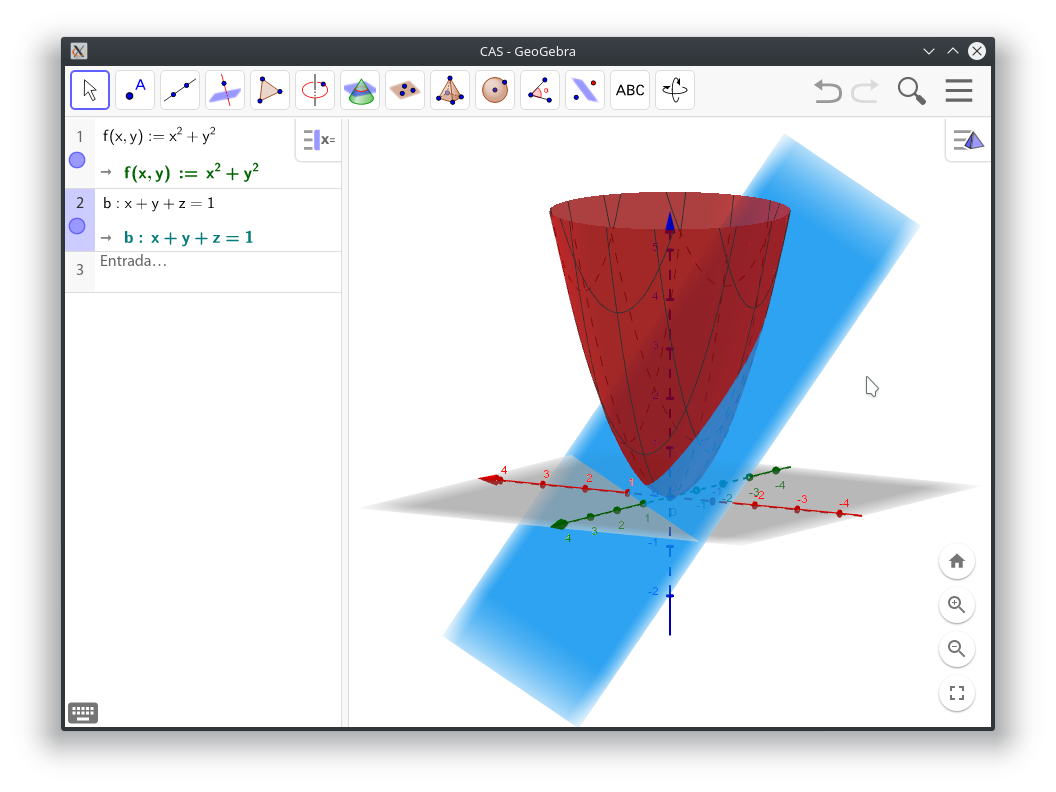
\includegraphics[width=\textwidth]{img/introduccion/3D-graphic-view}
\caption{Representaciones gráficas en la \field{Vista Gráfica 3D}.} \label{g:vista-grafica-3D}
\end{center}
\end{figure}

También es posible la representación de curvas paramétricas al igual que en el plano real, pero introduciendo el vector con las tres funciones coordenadas en función de un parámetro.
Por ejemplo, el comando \command{h(t):=(cos(t), sen(t), t/2)} dibuja la curva que se muestra en la figura~\ref{g:curva-parametrica-3D}.

\begin{figure}[h!]
\begin{center}
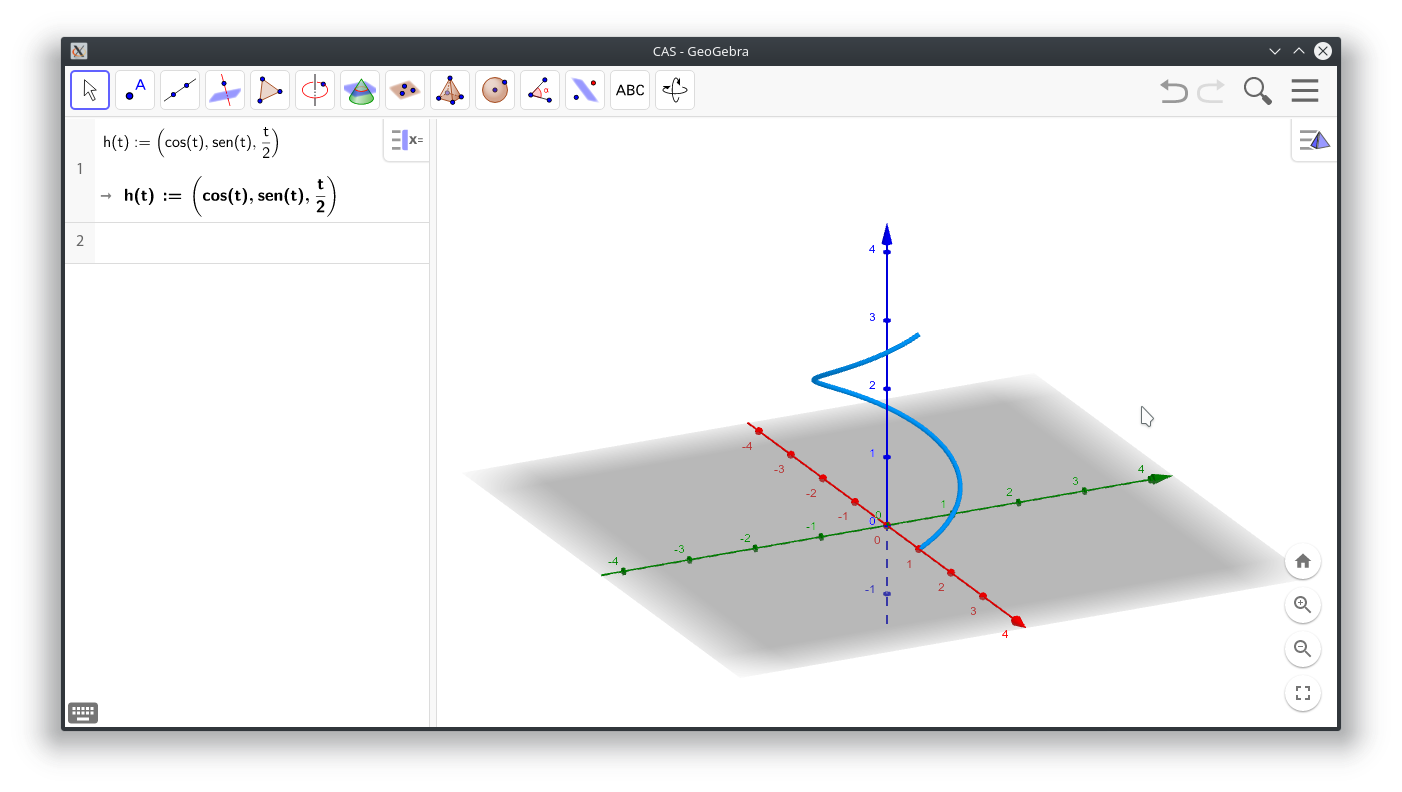
\includegraphics[width=\textwidth]{img/introduccion/3D-parametric-curve}
\caption{Representación de una curva paramétrica en el espacio.} \label{g:curva-parametrica-3D}
\end{center}
\end{figure}

Al igual que en la \field{Vista Gráfica}, es posible cambiar el aspecto de cualquier objeto geométrico haciendo clic con el botón derecho del ratón sobre él y seleccionando el menú \menu{Configuración} del menú contextual que aparece.
Esto abre un panel que permite cambiar el nombre del objeto, el color, el grosor o la transparencia del trazo, e incluso ponerle un rótulo que aparezca en la \field{Vista Gráfica} junto al objeto.

Del mismo modo, es posible hacer un zoom para acercar o alejar la vista haciendo clic en los botones 
\includegraphics[scale=0.03]{img/introduccion/zoom-in-button} y 
\includegraphics[scale=0.03]{img/introduccion/zoom-out-button} respectivamente.
También se puede mover la vista con el botón 
\includegraphics[scale=0.03]{img/introduccion/move-button} o rotarla con el botón 
\includegraphics[scale=0.03]{img/introduccion/rotate-button}.


\section{Gestión de archivos}
Las expresiones y los cálculos realizados dentro de la \field{Vista CAS} se pueden guardar en un archivo.

\subsection*{Guardar un archivo}
Para guardar las expresiones y los resultados de la \field{Vista CAS} se puede utiliza el menú \menu{Archivo>Guardar}.
Si no hemos iniciado sesión en el servidor de Geogebra nos preguntará el nombre de usuario y la contraseña para iniciar la sesión (ver figura~\ref{g:login}).
Si aún no se dispone de una cuenta de usuario es posible registrarse también en este momento, pero si no se desea identificarse se puede hacer clic en el enlace \command{Continuar sin identificarse ahora}.

\begin{figure}[h!]
\begin{center}
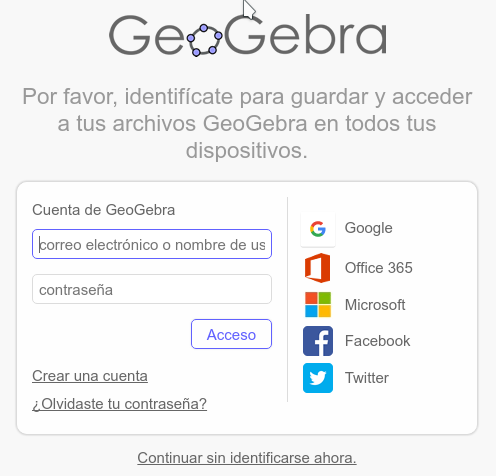
\includegraphics[scale=0.6]{img/introduccion/login}
\caption{Inicio de sesión en el servidor de Geogebra} \label{g:login}
\end{center}
\end{figure}

Si hemos iniciado sesión en el servidor, nos preguntará el nombre que queremos darle al archivo y se subirá automáticamente a la nube de Geogebra.
De este modo estará disponible en la web de Geogebra cuando nos conectemos con nuestro cuenta de usuario.

Si no se ha iniciado sesión en el servidor, entonces aparecerá un cuadro de diálogo donde podremos indicar el nombre que queremos darle al fichero y la seleccionar la carpeta donde queremos guardarlo.
Los archivos de geogebra tienen extensión \texttt{*.ggb}.

Una vez guardado el archivo, su nombre aparecerá en la barra de título de la ventana de Geogebra.


\subsubsection*{Abrir un archivo}
Para abrir un archivo de geogebra se utiliza el \menu{Archivo>Abrir}.
En el cuadro de diálogo que aparece se puede optar por abrir un archivo de la web de Geogebra, o bien abrir un archivo local.

En el caso de que hayamos iniciado sesión en el servidor, automáticamente aparecerán nuestros archivos de la nube de Geogegra.
Si no hemos iniciado sesión en el servidor entonces se puede abrir cualquier archivo público de la web de Geogebra.
Para ello podemos introducir cualquier término en la barra de búsqueda que aparece y nos aparecerán los archivos que incluyen esos términos.
Seleccionando cualquiera de ellos se descargará y se abrirá en Geogebra.

Si se desea abrir un archivo local hay que hacer clic en la carpeta que aparece y se abrirá un cuadro de diálogo donde debemos indicar el archivo que queremos abrir.


\section{Impresión}
Geogebra permite imprimir las vistas gráficas seleccionando el menú \menu{Previsualización}.
Tras esto aparece un cuadro de diálogo donde se puede seleccionar la ventana gráfica que se desea imprimir y las unidades de los ejes.
Finalmente aparece el cuadro de diálogo de las impresoras donde hay que seleccionar la impresora con la que se quiere imprimir.

También es posible exportar las vistas gráficas a diferentes formatos con el menú \menu{Descargar como}.
Si se desea imprimir además de las gráficos las expresiones de la \field{Vista CAS} hay que seleccionar la opción \option{Construcción dinámica con página web (html)}.
Esto genera una página web que puede abrirse con cualquier navegador y después imprimirse de la forma habitual.


\section{Ejercicios resueltos}
\begin{enumerate}
\item Introducir y evaluar las siguientes expresiones matemáticas.
      \begin{enumerate}
      \item $4x-\dfrac{1}{x}-5$.
            \begin{indication}
            Introducir la expresión \command{4x-1/x-5} en la \field{Barra de Entrada} de la \field{Vista CAS}.
            \end{indication}
      \item $\dfrac{4x-1}{x}-5$.
            \begin{indication}
            Introducir la expresión \command{(4x-1)/x-5} en la \field{Barra de Entrada} de la \field{Vista CAS}.
            \end{indication}
      \item $4x-\dfrac{1}{x-5}$.
            \begin{indication}
            Introducir la expresión \command{4x-1/(x-5)} en la \field{Barra de Entrada} de la \field{Vista CAS}.
            \end{indication}
      \item $\dfrac{4x-1}{x-5}$.
            \begin{indication}
            Introducir la expresión \command{(4x-1)/(x-5)} en la \field{Barra de Entrada} de la \field{Vista CAS}.
            \end{indication}
      \end{enumerate}

\item Definir los siguientes objetos matemáticos y dibujarlos.
      \begin{enumerate}
      \item Las constantes $a=2$ y $b=3$.
            \begin{indication}
            \begin{enumerate}
            \item Introducir el comando \command{a:=2} en la \field{Barra de Entrada} de la \field{Vista CAS} y activar la \field{Vista Gráfica}.
            \item Para dibujar el deslizador de la constante hacer clic sobre el círculo que aparece a la izquierda de la expresión anterior.
            \item Introducir el comando \command{b:=3} en la \field{Barra de Entrada}.
            \item Para dibujar el deslizador de la constante hacer clic sobre el círculo que aparece a la izquierda de la expresión anterior.
            \end{enumerate}
            \end{indication}
      \item La recta $f(x)=a+bx$.
            Utilizar los deslizadores de las constantes para ver cómo cambia la recta.
            \begin{indication}
            Introducir el comando \command{f(x):=a+b*x} en la \field{Barra de Entrada}.
            \end{indication}
      \item La ecuación $ax^2+by^2=8$.
            Utilizar los deslizadores de las constantes para ver cómo cambia la recta.
            \begin{indication}
            Introducir el comando \command{a*x\^{}2+b*y\^{}2=8} en la \field{Barra de Entrada}.
            \end{indication}
      \end{enumerate}

\item Definir las siguientes funciones y dibujarlas.
      \begin{enumerate}
      \item $f(x):=x^2$.
            \begin{indication}
            Introducir el comando \command{f(x):=x\^{}2} en la \field{Barra de Entrada} de la \field{Vista CAS} y activar la \field{Vista Gráfica}.
            \end{indication}
      \item $g(x):=\log(x)$.
            \begin{indication}
            Introducir el comando \command{g(x):=log(x)} en la \field{Barra de Entrada}.
            \end{indication}
      \item $h(x):=\sen(x)$.
            \begin{indication}
            Introducir el comando \command{g(x):=sen(x)} en la \field{Barra de Entrada}.
            \end{indication}
      \item $g\circ f(x)$.
            \begin{indication}
            Introducir el comando \command{g(f(x))} en la \field{Barra de Entrada} y hacer clic en el círculo que aparece a la izquierda de la expresión.
            \end{indication}
      \item $h\circ g \circ f(x)$.
            \begin{indication}
            Introducir el comando \command{h(g(f(x)))} en la \field{Barra de Entrada} y hacer clic en el círculo que aparece a la izquierda de la expresión.
            \end{indication}
      \item $f\circ g \circ h(x)$.
            \begin{indication}
            Introducir el comando \command{f(g(h(x)))} en la \field{Barra de Entrada} y hacer clic en el círculo que aparece a la izquierda de la expresión.
            \end{indication}
      \end{enumerate}

\item  Dadas las matrices
      \[
      A=\left(
      \begin{array}{cc}
      a_{11} & a_{12} \\
      a_{21} & a_{22} \\
      a_{31} & a_{32}
      \end{array}
      \right)
      \qquad
      B=\left(
      \begin{array}{ccc}
      1 & 2 & 3 \\
      4 & 5 & 6
      \end{array}
      \right)
      \]
      y el vector $v=(x, y, z)$, se pide:

      \begin{enumerate}
      \item Definir las matrices $A$ y $B$, y el vector $v$.
            \begin{indication}
            \begin{enumerate}
            \item Introducir el comando \command{A:=\{\{a\_{11},a\_{12}\},\{a\_{21},a\_{22}\},\{a\_{31},a\_{32}\}\}} en la \field{Barra de Entrada} de la \field{Vista CAS}.
            \item Introducir el comando \command{B:=\{\{1,2,3\},\{4,5,6\}\}} en la \field{Barra de Entrada}.
            \item Introducir el comando \command{v:=(x,y,z)} en la \field{Barra de Entrada}.
            \end{enumerate}
            \end{indication}
      \item Calcular $A\cdot B$.
            \begin{indication}
            Introducir el comando \command{A*B} en la \field{Barra de Entrada}.
            \end{indication}
      \item Calcular $B\cdot A$.
            \begin{indication}
            Introducir el comando \command{B*A} en la \field{Barra de Entrada}.
            \end{indication}
      \item Calcular $v\cdot A$.
            \begin{indication}
            Introducir el comando \command{v*A} en la \field{Barra de Entrada}.
            \end{indication}
      \item Calcular $B\cdot v$.
            \begin{indication}
            Introducir el comando \command{B*v} en la \field{Barra de Entrada}.
            \end{indication}
      \item Sustituir $x=1$, $y=1$ y $z=0$ en el vector anterior y dibujarlo.
            \begin{indication}
            Introducir el comando \command{Sustituye(\$,\{x=1,y=1,z=0\})} en la \field{Barra de Entrada} y hacer clic en el círculo que aparece a la izquierda de la expresión.
            \end{indication}
      \item Calcular el módulo del vector anterior.
            \begin{indication}
            Introducir el comando \command{|\$|} en la \field{Barra de Entrada} y hacer clic en el círculo que aparece a la izquierda de la expresión.
            \end{indication}
      \item Cambiar la sustitución anterior por $x=0$, $y=0$ y $z=1$ y observar cómo cambia el módulo del vector resultante.
            \begin{indication}
            Editar la línea de la sustitución anterior y cambiarla por  \command{Sustituye(\$,\{x=0,y=0,z=1\})} en la \field{Barra de Entrada}.
            \end{indication}
      \end{enumerate}

\item Encontrar los puntos donde se cortan las gráficas de las funciones $f(x)=x^2$ y $g(x)=\dfrac{x+1}{2}$ y dibujarlos.
      \begin{enumerate}
      \item Introducir el comando \command{f(x):=x\^{}2} en la \field{Barra de Entrada} de la \field{Vista CAS} y activar la \field{Vista Gráfica}.
      \item Introducir el comando \command{g(x):=(x+1)/2} en la \field{Barra de Entrada}.
      \item Para resolver la ecuación, introducir el comando \command{Resuelve(f=g)} en la \field{Barra de Entrada}.
      \item Para dibujar los puntos de intersección, introducir el comando \command{Interseca(f,g)} en la \field{Barra de Entrada} y hacer clic sobre el círculo que aparece a la izquierda de la expresión.
      \end{enumerate}

\item Dibujar la parametrizada
      \[
      g(t)=
      \begin{cases}
      \cos(t) \\
      2\sen(t)\cos(t)
      \end{cases}
      t\in \mathbb{R}
      \]

      \begin{indication}
      Introducir el comando \command{g(t):=(cos(t), 2sen(t)cos(t))} en la \field{Barra de Entrada} de la \field{Vista CAS} y activar la \field{Vista Gráfica}.
      \end{indication}

\item Representar gráficamente las siguientes superficies
      \[
            f(x,y)=\dfrac{\sen(x^2+y^2)}{\sqrt{x^2+y^2}}, \qquad x^2+y 2+(z-2)^2=1
            \]
      y la curva paramétrica
      \[
      h(t)=
      \begin{cases}
      \sen(t) \\
      \cos(t) \\
      t/2
      \end{cases}
      t\in \mathbb{R}
      \]
      \begin{indication}
      \begin{enumerate}
      \item Introducir el comando \command{f(x,y):=(sen(x\^{}2+y\^{}2/(sqrt(x\^{}2+y\^{}2)))} en la \field{Barra de Entrada} de la \field{Vista CAS} y activar la \field{Vista Gráfica 3D}.
      \item Introducir el comando \command{x\^{}2+y\^{}2+(z-2)\^{}2=1}  en la \field{Barra de Entrada}.
      \item Introducir el comando \command{h(t):=(sen(t),cos(t),t/2)}  en la \field{Barra de Entrada}.
      \end{enumerate}
      \end{indication}
\end{enumerate}